\newpage

\subsection*{Задание 4: Измерение частотной погрешности ваттметра} 


	При измерении мощности переменного тока определяют частотную и фазовую погрешности 			ваттметра Д535. Для определения частотной погрешности собирают схему изображенную на 	рисунке. \\
	\vspace{1.5cm}
 	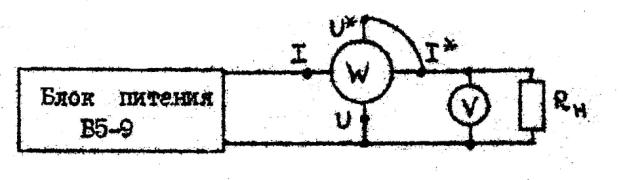
\includegraphics[width=\textwidth]{ch4.png}\\
 	
 	В качестве источника сигала используют генератор типа ГЗ-109, а в качестве нагрузки 		- магазин сопротивлений типа МСР (RН = 500 Ом). Ваттметр W типа Д535 устанавливают 			на предел измерения по току 50 мА и по напряжению - 75 В Изменяя выходное напряжение 	генератора, устанавливают напряжение на нагрузке, равное 30 В. Частоту генератора			изменяют в пределах от 20 Гц до 10 кГц, поддерживая постоянным напряжение на 				нагрузке, и регистрируют показания ваттметра.  \\
 	Результаты представлены в Форме 4:\\
 	
 	
 	\begin{table} [h!]
 	 \begin{tabular}{|p{4cm}|p{1cm}|p{1cm}|p{1cm}|p{1cm}|p{1cm}|p{1.2cm}|						p{1.2cm}|p{1.2cm}|p{1.2cm}|}
 	\hline
 	Напряжение $U_{H}$, (В) & 30 & 30 & 30 & 30 & 30 & 30 & 30 & 30 & 30 \\
 	\hline
 	Частота $f$, (Гц) & 20 & 50 & 100 & 200 & 500 & 1000 & 2000 & 5000 & 10000 \\
 	\hline
 	Мощность $P_{w}$, (Вт) & 2 & 2 & 2 & 2 & 2.05 & 2.05 & 2.1 & 2.1 & 1.95 \\
 	\hline
 	Погрешность $\delta _{f}$, (\%) & 0 & 0 & 0 & 0 & 25 & 25 & 50 & 50 & 25 \\
 	\hline
 	\end{tabular}
 	\end{table}
 	
 	
 	\vspace{1cm}
 	Частотную погрешность ваттметра рассчитывают по формуле:\\
 	$ \delta _{f} = |(P_{w} - P_{f0}) / P_{f0}| $ \\
 	где $P_{w}$ – показания ваттметра,\\
 	$P_{f0}$ – показания ваттметра на частоте f0 = 100 Гц.\\
 	
 	
  
  